% ------------------------------------------------------------------------------
% TYPO3 CMS 7.2 - What's New (English Version)
%
% @author	Michael Schams <schams.net>
% @license	Creative Commons BY-NC-SA 3.0
% @link		http://typo3.org/download/release-notes/whats-new/
% @language	English
% ------------------------------------------------------------------------------
% LTXE-CHAPTER-UID:		93899f32-8efb477e-ed6973d2-b679bd8e
% LTXE-CHAPTER-NAME:	Backend User Interface
% ------------------------------------------------------------------------------

\section{Backend / Внутренний интерфейс}
\begin{frame}[fragile]
	\frametitle{Backend / Внутренний интерфейс}

	\begin{center}\huge{Глава 1:}\end{center}
	\begin{center}\huge{\color{typo3darkgrey}\textbf{Backend / Внутренний интерфейс}}\end{center}

\end{frame}

% ------------------------------------------------------------------------------
% LTXE-SLIDE-START
% LTXE-SLIDE-UID:		600e206c-1a890374-a99a4149-9917d140
% LTXE-SLIDE-ORIGIN:	c151f95c-3fe3eb42-442ce244-5f987f80 English
% LTXE-SLIDE-TITLE:		Customized BE login form
% LTXE-SLIDE-REFERENCE:	unknown
% ------------------------------------------------------------------------------
\begin{frame}[fragile]
	\frametitle{Backend / Внутренний интерфейс}
	\framesubtitle{Настраиваемая форма авторизации}

	Системное расширение \texttt{backend} позволяет администраторам устанавливать
	фоновое изображение, логотип и цвет экрана авторизации во внутреннем интерфейсе:

	\begin{figure}
		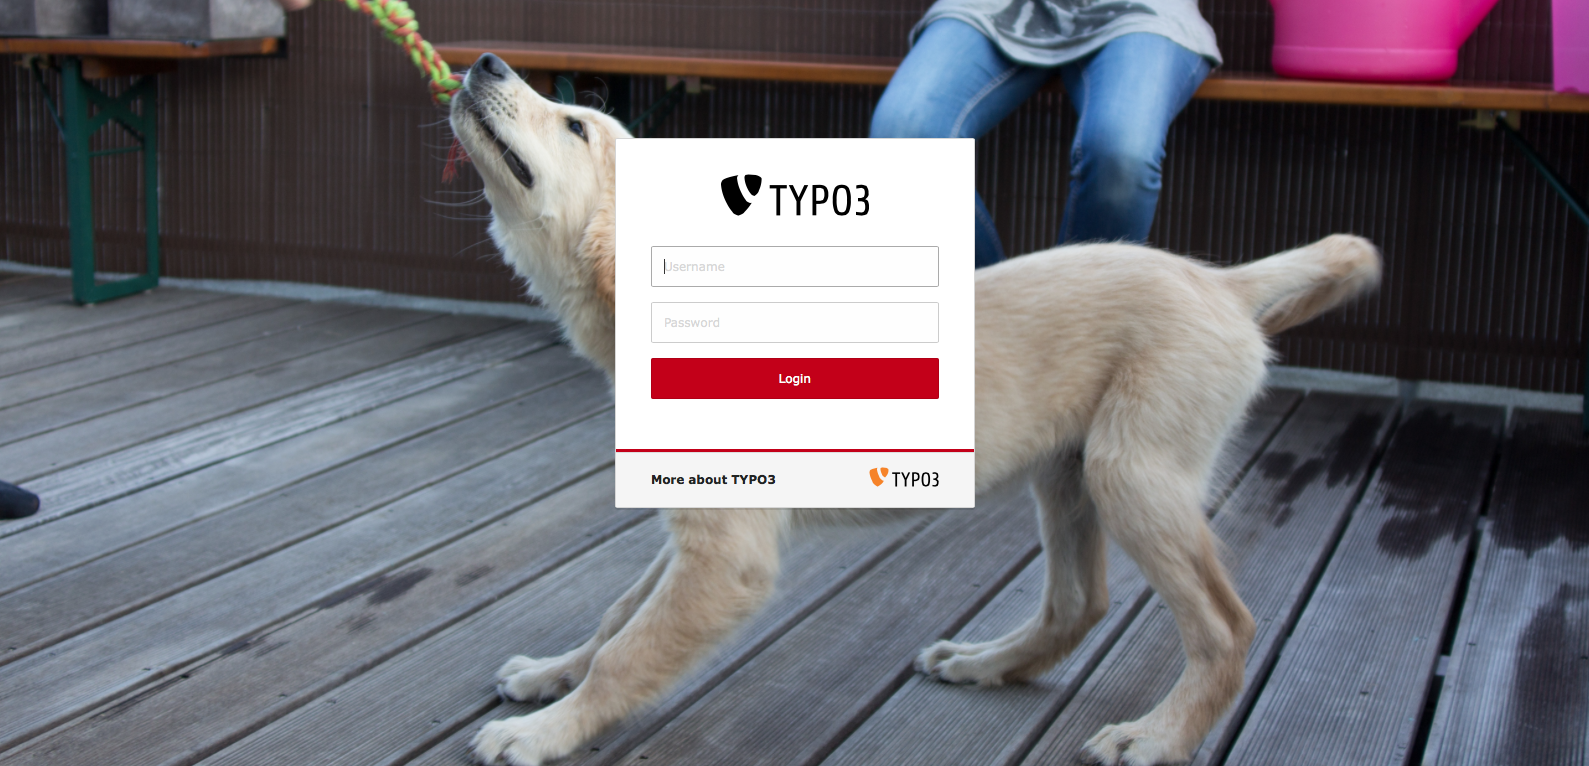
\includegraphics[width=0.75\linewidth]{BackendUserInterface/Login.png}
	\end{figure}

\end{frame}

% ------------------------------------------------------------------------------
% LTXE-SLIDE-START
% LTXE-SLIDE-UID:		d4ae9eb1-0e9177ab-a52c8d92-0a26fbbd
% LTXE-SLIDE-ORIGIN:	e2e353ae-3b2b5c00-0cd7c57d-d97d22c9 English
% LTXE-SLIDE-TITLE:		Add image cropping
% LTXE-SLIDE-REFERENCE:	Feature-65584-AddImageCropping.rst
% ------------------------------------------------------------------------------
\begin{frame}[fragile]
	\frametitle{Backend / Внутренний интерфейс}
	\framesubtitle{Работа с изображениями: обрезка}

	Функционал работы с изображениями позволяет редакторам обрезать изображения во
	 внутреннем интерфейсе. Эта возможность должна быть принудительно установлена
	  для пользователей внутреннего интерфейса ("Exclude Fields / Поля исключения"):

	\begin{figure}
		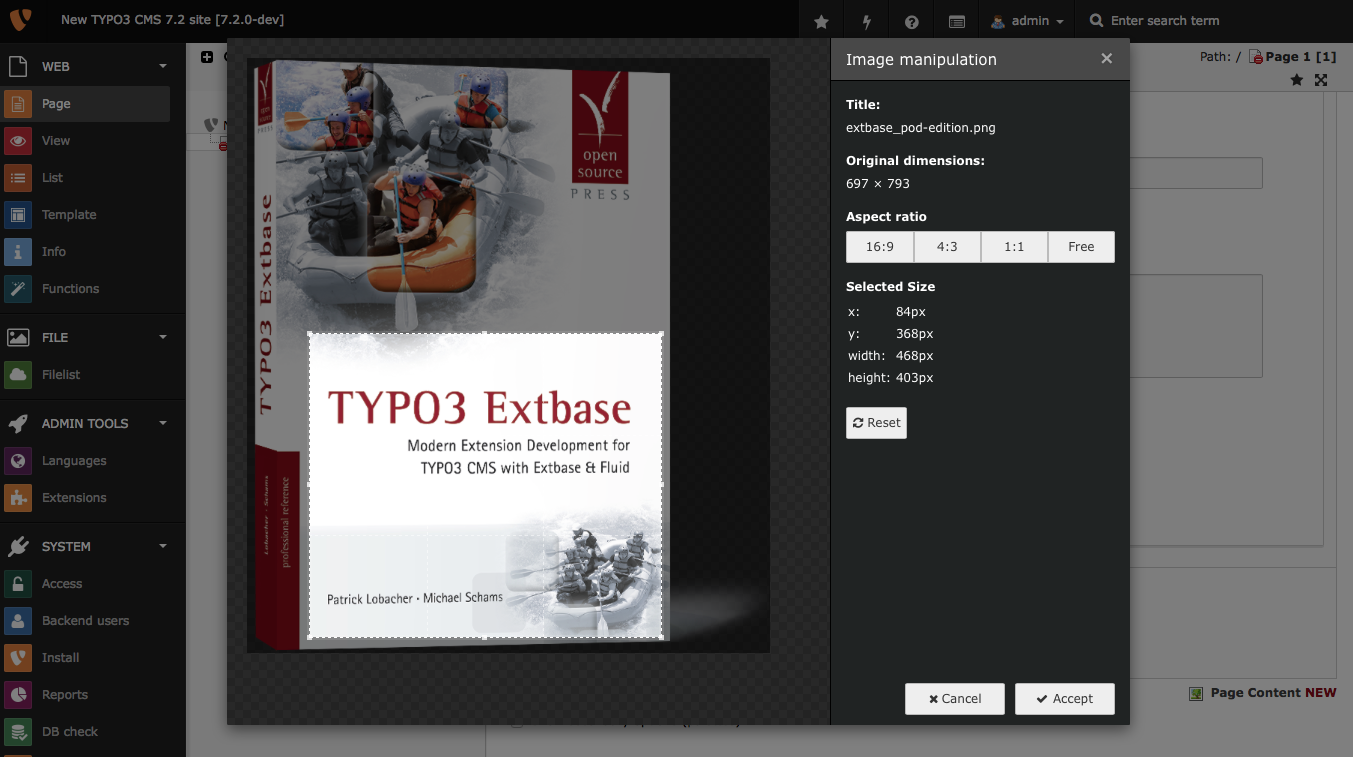
\includegraphics[width=0.7\linewidth]{BackendUserInterface/ImageCropping.png}
	\end{figure}

\end{frame}

% ------------------------------------------------------------------------------
% LTXE-SLIDE-START
% LTXE-SLIDE-UID:		1a4d539e-12989442-bed12bdb-6d023ed9
% LTXE-SLIDE-ORIGIN:	301dfea9-d2debf3e-dcaa7bcd-205e5990 English
% LTXE-SLIDE-TITLE:		Add backend user groups to backend user module
% LTXE-SLIDE-REFERENCE:	Feature-64686-AddBackendUserGroupsToBackendUserModule.rst
% ------------------------------------------------------------------------------
\begin{frame}[fragile]
	\frametitle{Backend / Внутренний интерфейс}
	\framesubtitle{Группы внутренних пользователей}

	Теперь управлять группами внутренних пользователей возможно из подмодуля модуля
	"Внутренние пользователи / Backend Users":

	\begin{figure}
		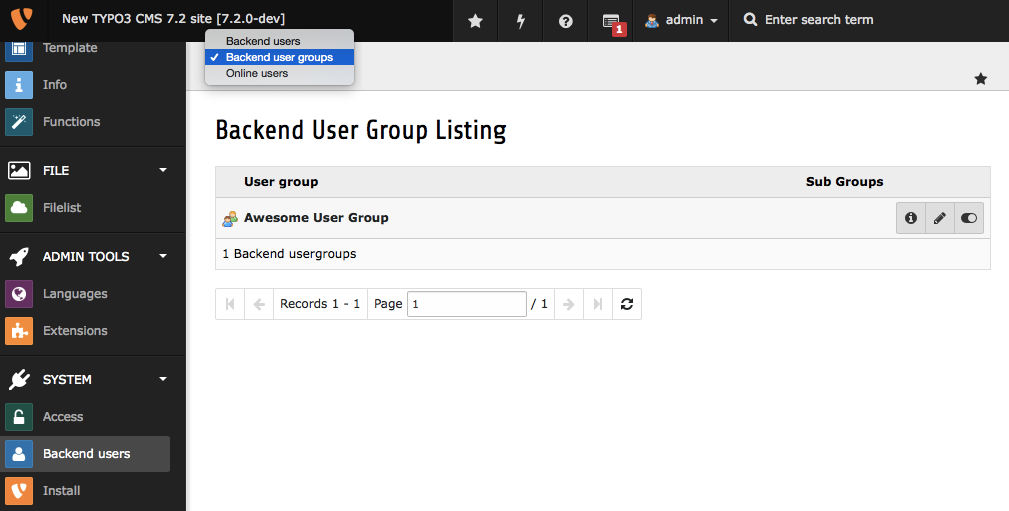
\includegraphics[width=0.70\linewidth]{BackendUserInterface/UserGroups.png}
	\end{figure}

\end{frame}

% ------------------------------------------------------------------------------
% LTXE-SLIDE-START
% LTXE-SLIDE-UID:		f8d3b946-774cc83c-b2fe3db3-1b577c85
% LTXE-SLIDE-ORIGIN:	daa83c1e-08d2716b-de74cbda-42361551 English
% LTXE-SLIDE-TITLE:		Extension Manager: Disable automatic installation
% LTXE-SLIDE-REFERENCE:	Feature-50501-DisableAutomaticExtInstallation.rst
% ------------------------------------------------------------------------------
\begin{frame}[fragile]
	\frametitle{Backend / Внутренний интерфейс}
	\framesubtitle{Отключение автоматической установки расширений}

	Администраторы могут настроить модуль Управления расширениями не устанавливать
	 загруженные расширения сразу же:

	\begin{figure}
		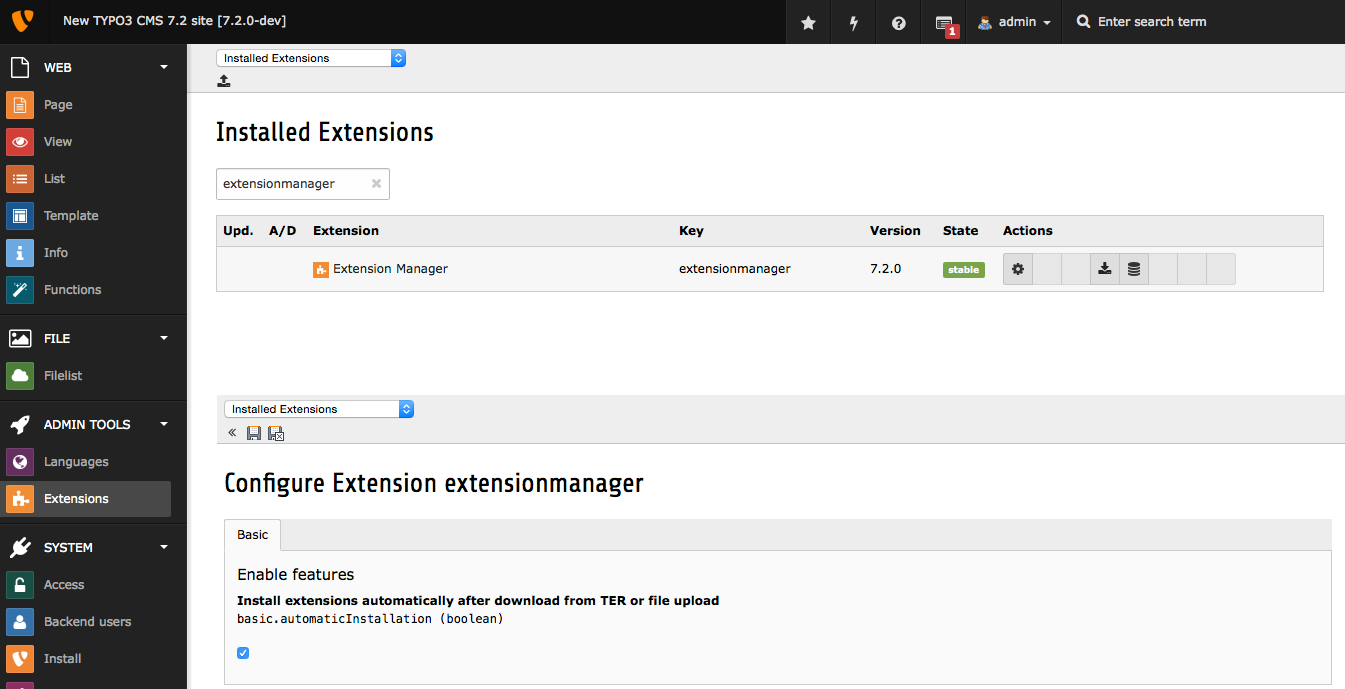
\includegraphics[width=0.70\linewidth]{BackendUserInterface/ExtManager.png}
	\end{figure}

\end{frame}

% ------------------------------------------------------------------------------
% LTXE-SLIDE-START
% LTXE-SLIDE-UID:		976d8173-6a4cee39-10616b50-83815ad0
% LTXE-SLIDE-ORIGIN:	20769920-da9df227-c3b527b9-9a23bac1 English
% LTXE-SLIDE-TITLE:		Show remaining characters below text fields
% LTXE-SLIDE-REFERENCE:	Feature-66029-ShowRemainingCharactersBelowTextFields.rst
% ------------------------------------------------------------------------------
\begin{frame}[fragile]
	\frametitle{Backend / Внутренний интерфейс}
	\framesubtitle{Оставшееся количество вводимых в текстовые поля символов}

	Количество оставшихся для ввода символов теперь отображается под текстовыми полями ввода:

	\begin{figure}
		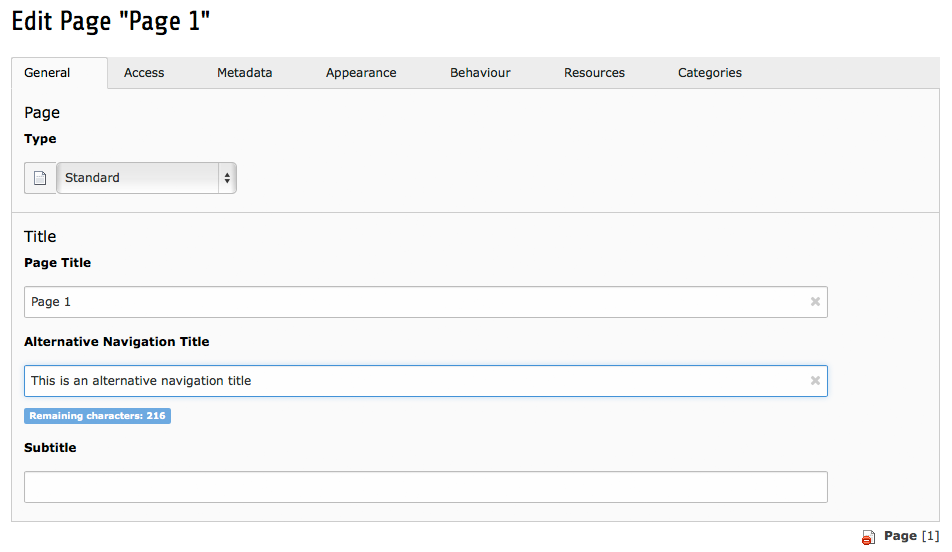
\includegraphics[width=0.70\linewidth]{BackendUserInterface/RemainingCharacters.png}
	\end{figure}

\end{frame}

% ------------------------------------------------------------------------------
% LTXE-SLIDE-START
% LTXE-SLIDE-UID:		540cdacb-b64595b1-9f9e6a6c-d5cf1b2e
% LTXE-SLIDE-ORIGIN:	ff760b86-9d6b1ecd-d0e98565-f23c51f0 English
% LTXE-SLIDE-TITLE:		Show confirm message on closing an editform with unsaved changes
% LTXE-SLIDE-REFERENCE:	Feature-65996-AddConfirmationOnCloseEditformWithUnsavedChanges.rst
% ------------------------------------------------------------------------------
\begin{frame}[fragile]
	\frametitle{Backend / Внутренний интерфейс}
	\framesubtitle{Подтверждение несохранённых изменений}

	Новый диалог напоминает редакторам о возможности потери несохранённых изменений:

	\begin{figure}
		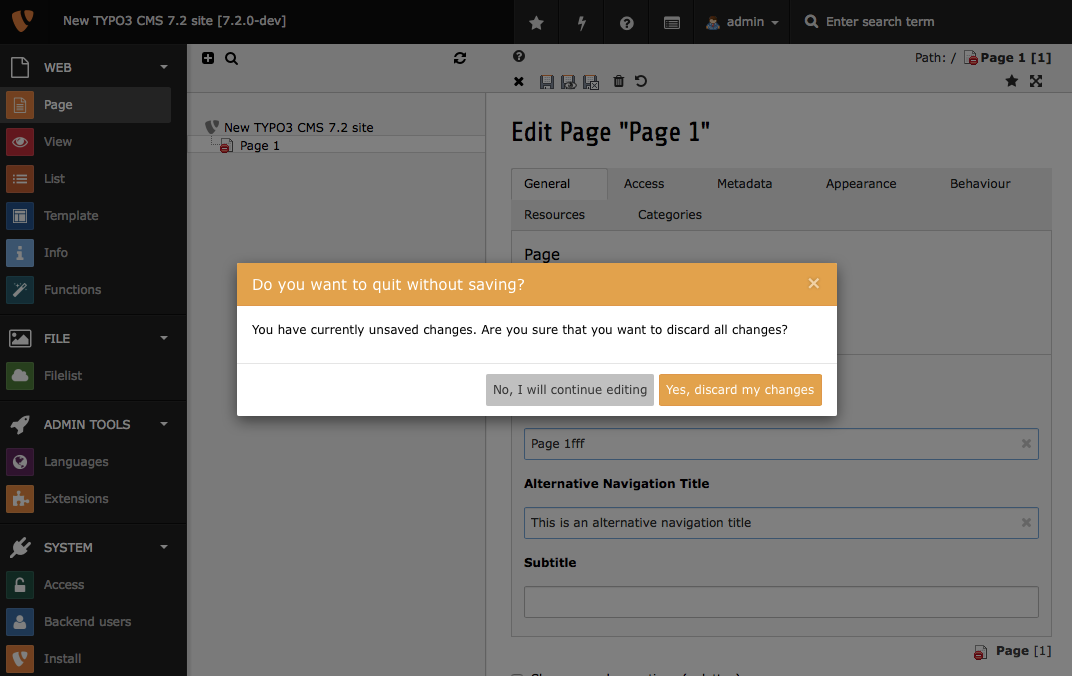
\includegraphics[width=0.65\linewidth]{BackendUserInterface/ClosingDialog.png}
	\end{figure}

\end{frame}

% ------------------------------------------------------------------------------
% LTXE-SLIDE-START
% LTXE-SLIDE-UID:		8f5dd2f4-11406386-4de1db92-4deee016
% LTXE-SLIDE-ORIGIN:	6ac9a35e-46541895-7509263e-28fb799f English
% LTXE-SLIDE-TITLE:		System Information Dropdown
% LTXE-SLIDE-REFERENCE:	Feature-65767-SystemInformationDropdown.rst
% ------------------------------------------------------------------------------
\begin{frame}[fragile]
	\frametitle{Backend / Внутренний интерфейс}
	\framesubtitle{Меню с системной информацией}

	Выпадающее меню выводит некую информацию об установленной системе TYPO3.
	Данные этого диалога можно дополнить:\newline
	\small(обратитесь к главе "Глубинные изменения")\normalsize

	\begin{figure}
		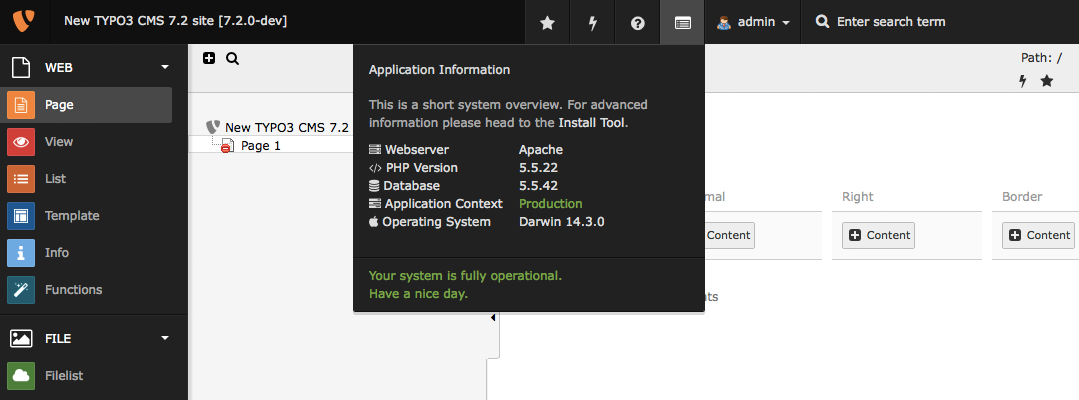
\includegraphics[width=0.85\linewidth]{BackendUserInterface/SystemInformation.png}
	\end{figure}

\end{frame}

% ------------------------------------------------------------------------------
% LTXE-SLIDE-START
% LTXE-SLIDE-UID:		f92a95a4-99e10e72-952e7551-42631325
% LTXE-SLIDE-ORIGIN:	79a2ee0c-3439d600-08990adb-6bed8c19 English
% LTXE-SLIDE-TITLE:		Ask for old password when changing
% LTXE-SLIDE-REFERENCE:	commit bf6f5226eb6cb441bb53657a88ef42f1cdb5155f
% ------------------------------------------------------------------------------
\begin{frame}[fragile]
	\frametitle{Backend / Внутренний интерфейс}
	\framesubtitle{Изменение пароля}

	Внутренние пользователи вынуждены изменить текущий (старый) пароль на новый:

	\begin{figure}
		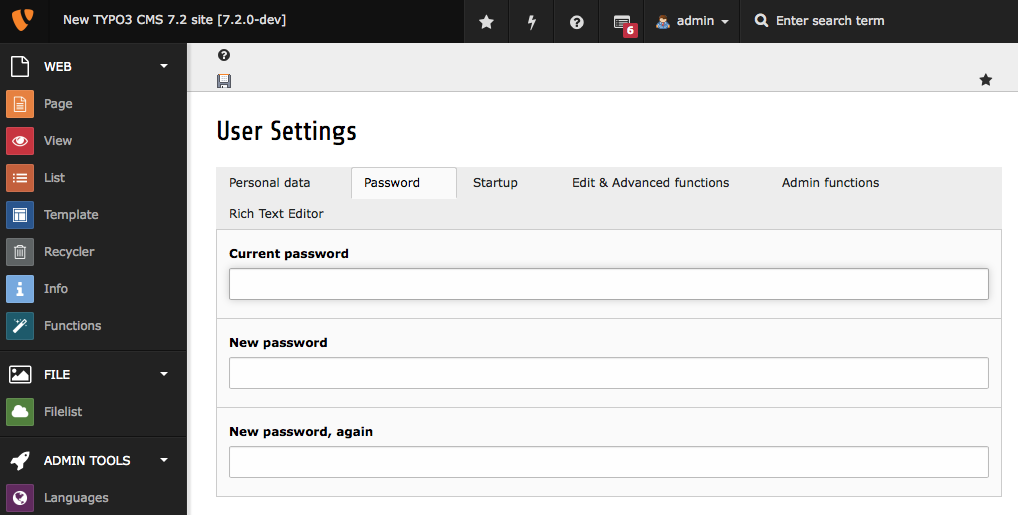
\includegraphics[width=0.7\linewidth]{BackendUserInterface/Password.png}
	\end{figure}

\end{frame}

% ------------------------------------------------------------------------------
% LTXE-SLIDE-START
% LTXE-SLIDE-UID:		7c1d636b-deb7f6f9-5724b771-bc2c0a8f
% LTXE-SLIDE-ORIGIN:	7725bce9-e606f055-bf2e7b4a-e870fe2a English
% LTXE-SLIDE-TITLE:		Add icon for "Show Content From Page"
% LTXE-SLIDE-REFERENCE:	commit f8aa3eea9aed97a901ef0c3e7c650e1218839596
% ------------------------------------------------------------------------------
\begin{frame}[fragile]
	\frametitle{Backend / Внутренний интерфейс}
	\framesubtitle{Значок страницы "Вывести содержимое со страницы / Show Content from Page"}

	Новый значок в дереве страниц для указания страниц, выводящих содержимое других страниц:

	\begin{figure}
		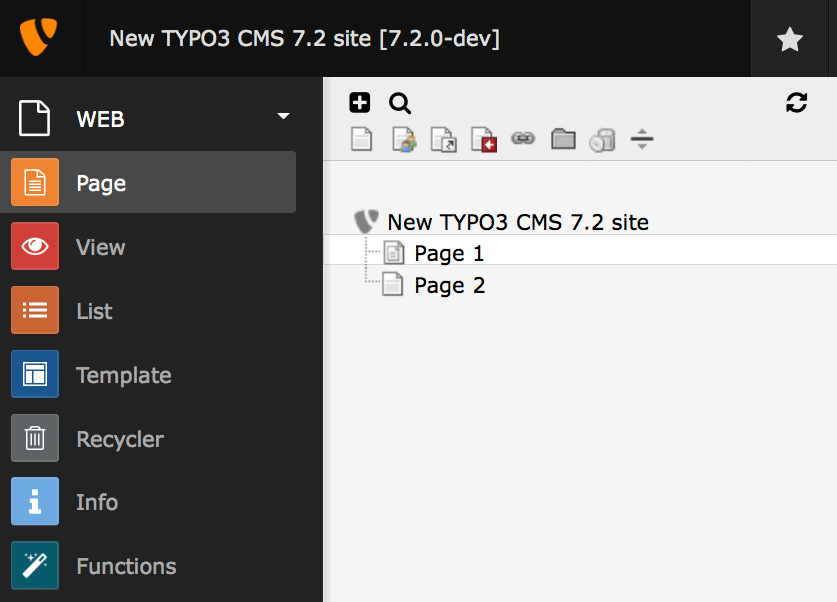
\includegraphics[width=0.45\linewidth]{BackendUserInterface/ShowContent.png}
	\end{figure}

\end{frame}

% ------------------------------------------------------------------------------
% LTXE-SLIDE-START
% LTXE-SLIDE-UID:		f5c47cc0-9e5730eb-cc93b447-18cdee2c
% LTXE-SLIDE-ORIGIN:	5ac2de45-9be12bf9-1c326192-602839fb English
% LTXE-SLIDE-TITLE:		Extension Manager: Choose version for update
% LTXE-SLIDE-REFERENCE:	commit a26396a4530b530744ec8b36c5fb5606789a6739
% ------------------------------------------------------------------------------
\begin{frame}[fragile]
	\frametitle{Backend / Внутренний интерфейс}
	\framesubtitle{Обновление расширений}

	При обновлении расширений теперь есть возможность выбора нужной версии:

	\begin{figure}
		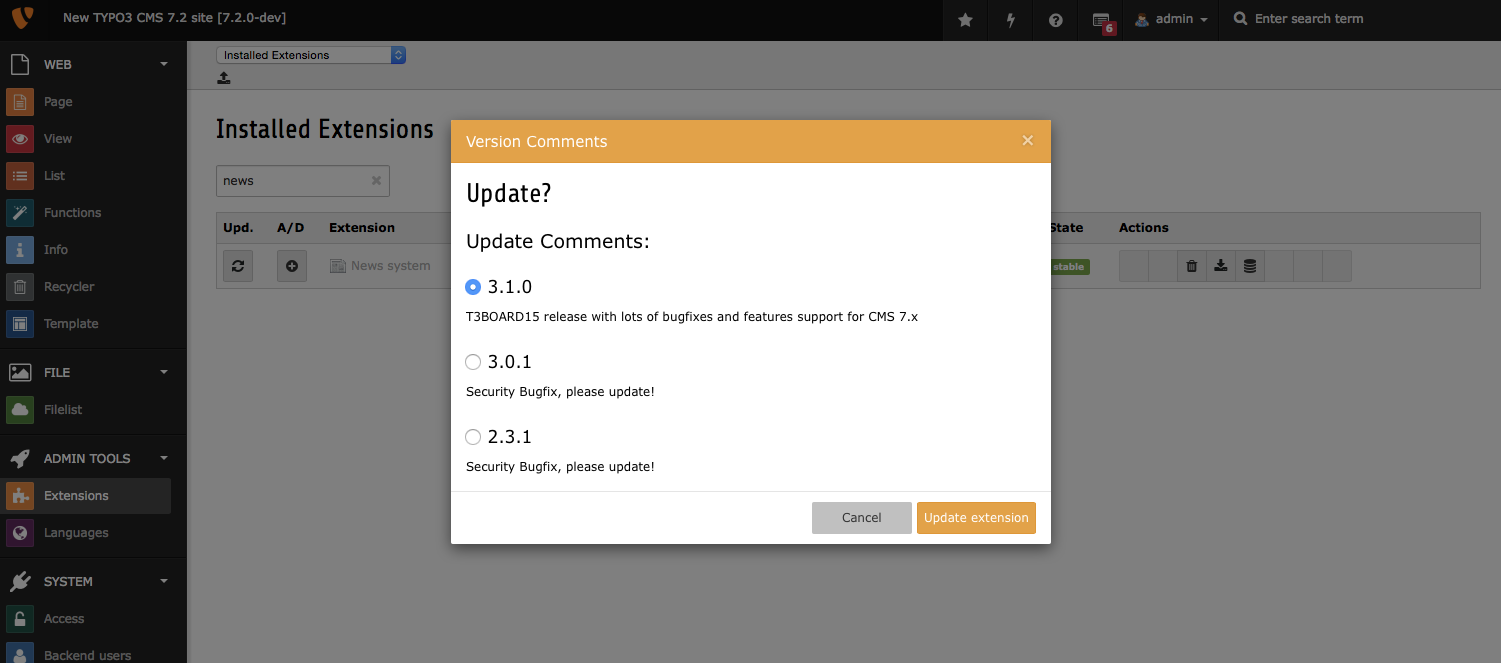
\includegraphics[width=0.9\linewidth]{BackendUserInterface/Update.png}
	\end{figure}

\end{frame}

% ------------------------------------------------------------------------------
% LTXE-SLIDE-START
% LTXE-SLIDE-UID:		0a66e9b2-31835b86-5fdd2e22-0be18fa1
% LTXE-SLIDE-ORIGIN:	f6be31f7-155d676c-0e551545-3fc89e89 English
% LTXE-SLIDE-TITLE:		Add scheduler task to remove deleted records
% LTXE-SLIDE-REFERENCE:	Feature-32651-AddSchedulerTaskToRemoveDeletedRecords.rst
% ------------------------------------------------------------------------------
\begin{frame}[fragile]
	\frametitle{Backend / Внутренний интерфейс}
	\framesubtitle{Задача для Корзины / Recycler}

	Новая задача в планировщике для системного расширения \texttt{recycler} удаляет
	помеченные как удалённые записи из таблиц базы данных. В задаче настраиваются
	максимальный возраст и задействованные таблицы.
	\newline
	То же может быть применимо и к файлам, если на них ссылаются в элементе содержимого.

	\begin{figure}
		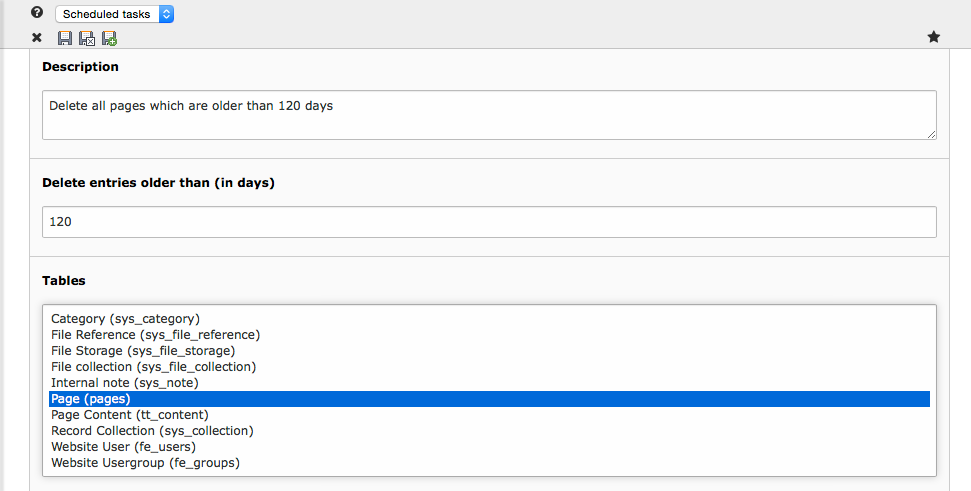
\includegraphics[width=0.68\linewidth]{BackendUserInterface/RecyclerTask.png}
	\end{figure}

\end{frame}

% ------------------------------------------------------------------------------
